
\chapter{Introducción}

\section{Antecedentes históricos}
El ser humano, en la década del 60, ante la incipiente necesidad de saber su posición en el planeta desarrolló un sistema de posicionamiento  llamado OMEGA y posteriormente otro llamado TRANSIT o \ac{NAVSAT}, que  fue resultado del trabajo conjunto de la NASA y el departamento de defensa de los Estados Unidos. Años después este acabó siendo reemplazado debido a la falta de precisión que este tenía, y que alcanzaba un error de hasta 250 metros.

Su sucesor apareció en la década del 70 bajo el nombre de \ac{GPS} y su precisión permitía posicionar un objeto con un error de menos de 5 metros. Esto a través del cálculo del tiempo que tarda en llegar la señal al receptor, es decir, el efecto Doppler.

Funciona actualmente con un mínimo de 24 satélites en órbita sobre la tierra cuyas trayectorias sincronizadas le permiten mapear completamente el planeta y entregar posicionamiento casi exacto a dispositivos móviles y vehículos.

Existen desde ya hace décadas intentos por emular lo logrado con el GPS, pero para espacios interiores, estos intentos han recibido el nombre de \ac{IPS}, que conforme a lo que se presentará en capítulos posteriores han logrado obtener resultados de posición con márgenes de error inferiores a los 3 m. 

\section{Definición del problema}
Las condiciones bajo las cuales es posible para la señal propagarse no se cumplen en todos los ambientes. Existen lugares en que a diferencia de lo que sucede en el exterior, donde la señal se refleja haciendo posible la triangulación de la posición, esta se absorbe parcial o completamente y principalmente corresponden a espacios interiores, tales como una bodega, un centro comercial o una oficina, haciendo que posicionarse dentro de estos espacios sea imposible a través del GPS, es por esto que a fin de brindar nuevas experiencias a usuarios a través del posicionamiento dentro de estos espacios se han desarrollado soluciones utilizando la banda de los 2.4 [GHz] que es la utilizada por, entre otros tecnologías, el Wi-Fi. 

Esta ha sido ampliamente estudiada debido a la alta penetración comercial que ha alcanzado precisamente en estos espacios donde el GPS no da cobertura, sin embargo, dentro de los distintos enfoques en que se han abordado los estudios se tiene que la medición de los niveles de potencia radiada desde los \ac{AP}, a través de los cuales se realiza la triangulación de la posición, se ven altamente afectados por la variación del escenario caracterizado. Este tipo de variaciones pueden ser inducidas por la presencia de personas u objetos que reflejen o absorban la señal.

Es por esto que el método a través del cual se de solución al problema del posicionamiento en interiores debe ser un \ac{IPS} capaz de compensar la incidencia de estas variaciones en el \ac{RSSI} dentro de la operación del algoritmo y así, estimar correctamente la posición de objetivo deseado identificable a través de su dirección de \ac{MAC}.

\section{Estado del arte}

En cuánto a los enfoques que se han considerado para evaluar la posición de un dispositivo móvil en un espacio interior se han podido desarrollar diversas soluciones que apuntan de una u otra manera a aproximaciones geométricas. A fin de ordenar según la técnica, la documentación consultada, se hará una clasificación y dentro de las categorías, explicará las investigaciones en el área.\\

%%%%%%%%%%%%%%%%%%%%%%%%%%%%%%%%%%%%%%%%%%%%%%%%%%%%%%%%%%
                \clearpage 
%%%%%%%%%%%%%%%%%%%%%%%%%%%%%%%%%%%%%%%%%%%%%%%%%%%%%%%%%%

Se abordará siguiendo el esquema que está a continuación:
\begin{figure}[h!]
    \centering
    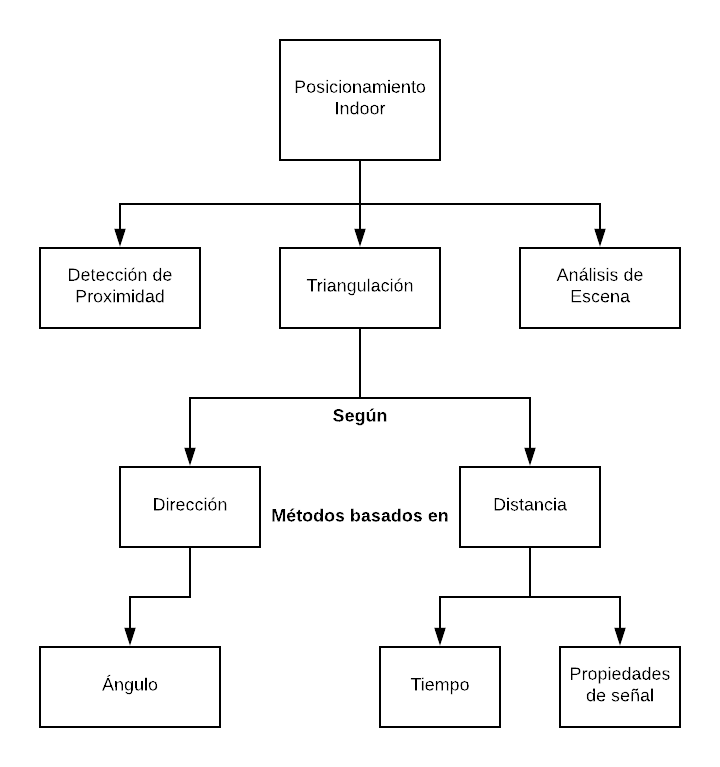
\includegraphics[scale = 0.3]{./images/diagrama}
    \label{fig:diagrama}
\end{figure}

%\begin{itemize}
%\item{\ac{AoA}: Referido, como su nombre lo dice, se refiere al ángulo de llegada de la señal del dispositivo móvil, proveniente de una ubicación desconocida, la cual es recibida en múltiples estaciones base. Resultaría provechoso un sistema de posicionamiento de este tipo puesto que solo requiere dos AP o Beacons, cuya precisión puede ser mejorada por la inclusión de un tercero. \\

%En este caso, y tal y como explican \textit{Kyle Davies e Ian Jones }en \cite{11}, si se incluye un tercer elemento se habla de triangulación:

%\begin{itemize
%\item{\textbf{Triangulación:} Este método, explicado en \textit{Recent Advances in Wireless Indoor Localization Tecniques and System}\cite{6} usa herramientas geométricas de triángulos para determinar la ubicación del objetivo. Tiene a su vez dos posibles variaciones:

% Trilateración: Si es que en lugar de usar propiedades geométricas de triángulos, utiliza círculos que corresponden al área de cobertura del AP. Estos a través de un punto de intersección de las circunferencias permiten estimar la posición del objetivo. Se basa en el nivel de RSS. Esto fue utilizado en \cite{3}, \cite{4}, \cite{5}, \cite{7}, \cite{8} y \cite{9}.}
% \end{itemize}

% En estos papers, específicamente en el trabajo de Zahid, Rosdiadee y Mahamod, ellos recopilaron información detallada sobre las técnicas de posicionamiento indoor a la fecha de publicación, hacen una diferencia respecto cuándo usar Trilateración o Triangulación, mencionando que cuando se trata de técnicas de medición de propagación basadas en tiempo, esto es \ac{ToF}, RTOF y TDOA o en RSS, se puede usar un algoritmo del tipo Trilateración, mientras que si se trata de AoA, el algoritmo a usar es el de Triangulación. 

% Sin embargo, esta aproximación depende del uso de antenas altamente directivas o bien, de arreglos de antenas lo que ciertamente aumenta sustancialmente el costo de su implementación. Ya que lo que se usa son relaciones geométricas que permiten estimar el punto de intersección. }

% \item{\ac{ToF}, este concepto está referido a la técnica a través de la cual se realizan cálculos de posición a través del tiempo de llegada de la señal respecto de diversos puntos de referencia.}
% \end{itemize}

% No obstante, las técnicas más usadas dentro de las consultadas en la revisión bibliográfica son aquellas que usan un método combinado de herramientas matemáticas del tipo estadísticas, en conjunto con los valores de RSS, para estimar la posición. Las herramientas son utilizadas para corregir errores que se producen en la recepción de la señal y que se originan en las reflexiones que esta experimenta a través del viaje desde y hacia el dispositivo.

% Se reconocen además dos fases muy bien definidas en el proceso de desarrollo de un sistema de posicionamiento. Una fase \textit{offline}, que guarda relación con el mapeo o la caracterización del espacio en función de los valores de intensidad de señal recibida en los cuadrantes en que se divide el espacio sobre el cual se moverá el dispositivo, y una fase \textit{online}, que es en la cual el dispositivo movil se mueve a través de este espacio enviando los RSSI a un servidor que consulta en la base de datos obtenida previamente, cuál es o debería ser la posición de este en el espacio.

% Sin embargo, sugieren autores en \cite{8}, \cite{11}, \cite{12} y \cite{14}, que la precisión mejora considerablemente, al rededor de un 45\% sobre los resultados preliminares, si es que se considera la media y la desviación estándar en los resultados.

%%%%%%%%%%%%%%%%%%%%%%%%%%%%%%%%%%%%%%%%%%%%%%%%%%%%%%%%%%
                \clearpage 
%%%%%%%%%%%%%%%%%%%%%%%%%%%%%%%%%%%%%%%%%%%%%%%%%%%%%%%%%%

\section{Hipótesis de trabajo}
\begin{center}
\textit{''Es posible posicionar un dispositivo, identificable a través de su MAC, en un espacio interior utilizando una \ac{NN} para compensar las variaciones de RSS de los \ac{AP} usados en la trilateración''}
\end{center}

\section{Objetivos}
A continuación se señalan los objetivos que apuntan a resolver el problema presentado y a probar la hipótesis de trabajo.

\subsection{Objetivo general}
Posicionar un dispositivo móvil, reconocible a través de su \ac{MAC} dentro de un espacio interior, a través de algoritmos de trilateración y \ac{NN}.

%\section{Objetivos específicos}
%\begin{enumerate}
%\item{a}
%\end{enumerate}

\section{Alcances y limitaciones}
El alcance de este proyecto estará limitado a encontrar la posición de un dispositivo móvil dentro del espacio del segundo piso de Edificio Tecnológico Mecánico de la Universidad de Concepción. Se ejecutará el algoritmo desarrollado en una laptop personal, utilizando Raspberry Pi como \ac{AP} y el resultado del posicionamiento se desplegará en una interfaz gráfica desarrollada en python.

\section{Metodología}

Para lograr posicionar un dispositivo móvil dentro del espacio interior, se buscará en primera instancia extraer los datos de RSSI obtenidos desde las tarjetas de Red de las placas. Posterior a esto se caracterizará el espacio de trabajo con sus respectivos niveles de RSS. Estas serán usadas para entrenar un modelo que, a través de RNN, pueda detectar la posición en que se halla un usuario, respecto de los niveles de potencia y la certidumbre que arroje el entrenamiento realizado. Finalmente, el resultado será desplegado en una interfaz gráfica.